\documentclass[a4paper,onecolumn,10pt]{article}
\usepackage[polish]{babel}
\usepackage[utf8]{inputenc}
\usepackage[T1]{fontenc}
\usepackage[left=2.1cm,right=2.1cm]{geometry}
\usepackage[dvipsnames]{xcolor}
\usepackage{amsmath,calc,indentfirst,fancyhdr,amsfonts,graphicx,epstopdf,caption, mathcomp, subcaption,wrapfig, siunitx,pbox,float,algorithm}
\usepackage[noend]{algpseudocode}


\makeatletter
\def\BState{\State\hskip-\ALG@thistlm}
\renewcommand{\ALG@name}{Algorytm}
\makeatother

\renewcommand{\baselinestretch}{1.1}	 % odstep miedzy liniami
\addto\captionspolish{\renewcommand{\figurename}{Wykres}} % zmiana podpisu pod obrazkami, zamiast "Rysunek" bedzie "Wykres"
\newcommand{\NN}{\mathbb{N}}			 % makro do znaku liczb naturalnych

\newcommand{\R}[1]{\textcolor{red}{#1}}  % makro do polecenia z parametrami - tutaj 1 parametr
\newcommand{\G}[1]{\textcolor{green}{#1}} 
\newcommand{\B}[1]{\textcolor{RoyalBlue}{#1}} 
% kolorowanie {\B{argument}}

\newcommand{\PICTURES}{} % szybsza kompilacja dzieki stalej "usuwajacej" obrazki
						 % zakomentowanie \PICTURES powoduje znikniecie obrazkow

\pagestyle{fancy} % formatuj caly dokument
\fancyhead{}
\fancyfoot{}
\renewcommand{\headrulewidth}{0pt}
\fancyfoot[R]{\thepage} % dla stron poza tytulowa nr w prawym dolnym rogu

\fancypagestyle{plain}{ % dla strony tytulowej nr w prawym dolnym rogu
	
	\renewcommand{\headrulewidth}{0pt}
	\fancyhf{}
	\fancyfoot[R]{\thepage}
}
% 17 linia w preamble.tex

\renewcommand{\arraystretch}{1.2}

\title{\Large\vspace{-2.5cm}{\Huge S}PRAWOZDANIE - LABORATORIUM NR {\Huge11}\\
	\textbf{Odszumianie sygnału przy użyciu FFT - splot funkcji} } 
\date{\Large30 maja 2019}
\author{\Large Marek Kiełtyka}

\begin{document}
\maketitle

\vspace{-1.2cm}\section{Wstęp}

\subsection{Szybka transformacja Fouriera (FFT – Fast Fourier Transform)}

Jest to algorytm pozwalający obliczyć dyskretną transformatę Fouriera (DFT) oraz transformatę do niej odwrotną w wydajny sposób. Stosuje się ją w licznych problemach numerycznych takich jak interpolacja, aproksymacja, szybkie mnożenie oraz rozwiązywanie równań różniczkowych. 

Porównując jej efektywność do klasycznej metody DFT jest wykorzystywana również do cyfrowego przetwarzania sygnału (odszumianie), kompresji danych (transformata cosinusowa) oraz analizy sygnałów czasowych. Na laboratorium szczególnie skupiono się na pierwszym aspekcie.

\subsection{Algorytm Cooleya-Tukeya (Radix-2)}

Wydajna i zarazem najprostsza implementacja FFT została opracowana w latach 60. XX wieku w celu szybkiej analizy danych sejsmologicznych. Należy w niej wyznaczyć współczynniki klasycznej DFT, lecz przy jak najmniejszym nakładzie obliczeniowym.

Zakłada się, że całkowita liczba węzłów jest potęgą liczby 2:
\begin{equation}
N = 2^r, \quad r \in \mathbb{N},
\end{equation}
które określamy w poniższy sposób.
\begin{equation}
x_j = \frac{2\pi}{N}j, \quad j = 0, 1, 2, \dots, N -1
\end{equation}
Przepis na współczynniki jest następujący
\begin{equation}
c_k = \left< E_k, f \right> = \sum_{j=0}^{N-1}f(x_j) E_k^{*} (x_j) = \sum_{j=0}^{N-1} f(x_j) \exp(-Ix_jk) = \sum_{j=0}^{N-1} f_j \exp \bigg( -I \frac{2\pi}{N}jk \bigg).
\end{equation}
Należy zgrupować osobno składniki parzyste ($j = 2m $) oraz nieparzyste ($j=2m+1$)
\begin{equation}
c_k = \sum_{m=0}^{\frac{N}{2} -1} f_{2m} \exp \bigg( -I \frac{2\pi}{N}(2m)k \bigg)  +
\sum_{m=0}^{\frac{N}{2} -1} f_{2m+1} \exp \bigg( -I \frac{2\pi}{N}(2m+1)k \bigg) 
\end{equation}
a następnie przekształcić do postaci
\begin{equation}
c_k = \sum_{m=0}^{\frac{N}{2} -1} f_{2m} \exp \bigg( -I \frac{2\pi}{N/2}mk \bigg)  +
\exp \bigg( -I\frac{2\pi}{N} k\bigg) \sum_{m=0}^{\frac{N}{2} -1} f_{2m+1} \exp \bigg( -I \frac{2\pi}{N/2}mk \bigg).
\end{equation}
Dla wygody wprowadza się oznaczenia
\begin{equation}
p_k = \sum_{m=0}^{\frac{N}{2} -1} f_{2m} \exp \bigg( -I \frac{2\pi}{N/2}mk \bigg),
\end{equation}
\begin{equation}
q_k =\sum_{m=0}^{\frac{N}{2} -1} f_{2m+1} \exp \bigg( -I \frac{2\pi}{N/2}mk \bigg) ,
\end{equation}
\begin{equation}
\varphi = \exp \bigg( -I\frac{2\pi}{N} k\bigg).
\end{equation}
Ostatecznie otrzymuje się wygodną postać
\begin{equation}
c_k = p_k + \varphi_k q_k,
\end{equation}
a biorąc pod uwagę okresowość można zauważyć związki:
\begin{equation}
p_{k+N/2} = p_k, \quad \quad q_{k+N/2} = q_k, \quad \quad \varphi_{k+N/2} = - \varphi_k,
\end{equation}
co automatycznie skraca czas obliczeń - wystarczy znaleźć tylko połowę ilości współczynników.
\\Oszczędność czasu bierze się z faktu, iż
\begin{equation}
c_k = 
\begin{cases}
p_k + \varphi_k q_k \quad &k < \frac{N}{2}\\
p_{k -\frac{N}{2}} - \varphi_k q_{k -\frac{N}{2}}, \quad &k \geq \frac{N}{2}
\end{cases}
\end{equation}
zatem wyznacza się tylko współczynniki dla $ k < \frac{N}{2} $.\\
Dalsze kroki algorytmu opierają się na podziale sum w $ p_k $ oraz w $ q_k $ na sumy zawierające tylko elementy parzyste i nieparzyste. Liczba elementów w każdej z dwóch powstałych sum jest wtedy dwukrotnie mniejsza niż w elemencie macierzystym. Proces rekurencyjnego podziału należy zakończyć, gdy liczba elementów jest równa 1.

\section{Zadanie do wykonania}

\subsection{Opis problemu}

Celem laboratorium było odszumienie pierwotnie zaszumionego sygnału $ f(t) $ z użyciem opisywanej metody. Jej omówione aspekty zostały uprzednio zaimplementowane w ciałach funkcji $$ gsl\_fft\_complex\_radix2\_forward,\quad gsl\_fft\_complex\_radix2\_backward $$ przez twórców biblioteki numerycznej \textit{GSL}. Przyjęty sygnał zaburzony postaci
\begin{equation}
f(t) = f_0 (t) + \Delta, \quad \Delta \in (-−0.5,0.5]
\end{equation}
korzystający z sygnału niezaburzonego
\begin{equation}
f_0 (t) = \sin (\omega t) + \sin (2\cdot \omega t) + \sin(3\cdot \omega t)
\end{equation}
należało odszumić z użyciem wyznaczonego uprzednio splotu dwóch funkcji definiowanego jako
\begin{equation}
(f * g) (t) = \int_{-\infty}^{\infty} f(\tau) g(t - \tau) \mathrm{d} \tau.
\end{equation}
Do wyznaczania współczynników wagowych zadano funkcję gaussowską
\begin{equation}
g(t) = \frac{1}{\sigma \sqrt{2\pi}} \exp \bigg(-\frac{t^2}{2\sigma^2} \bigg).
\end{equation}
\newpage
Założono parametry:
\begin{itemize}
	\item \makebox[2.2cm]{$ \omega = \frac{2\pi}{T}$} - pulsacja 
	\item \makebox[2.2cm]{$\Delta \in [-0.5, 0.5]$} - liczba pseudolosowa użyta do zaszumiania
	\item \makebox[2.2cm]{$N = 2^k$} - całkowita liczba węzłów, gdzie $k=8, 10, 12$
	\item \makebox[2.2cm]{$T = 1.0$} - okres
	\item \makebox[2.2cm]{$t_{max} = 3T$} - maksymalny okres rejestracji sygnału 
	\item \makebox[2.2cm]{$ dt = \frac{t_{max}}{N} $} - krok czasowy 
	\item \makebox[2.2cm]{$\sigma = \frac{T}{20}$}
\end{itemize}

\subsection{Wyniki}

Korzystając z programu napisanego w języku C++ i biblioteki \textit{GSL} (funkcje wykonujące transformatę Fouriera) sporządzono wykresy dla trzech przypadków. Kolejno na każdym przedstawiono razem sygnał zaburzony i niezaburzony, a także wynikowy splot funkcji, będący de facto sygnałem odszumionym. Wyniki zaprezentowano poniżej.
\begin{figure}[h!]
	\begin{center}
		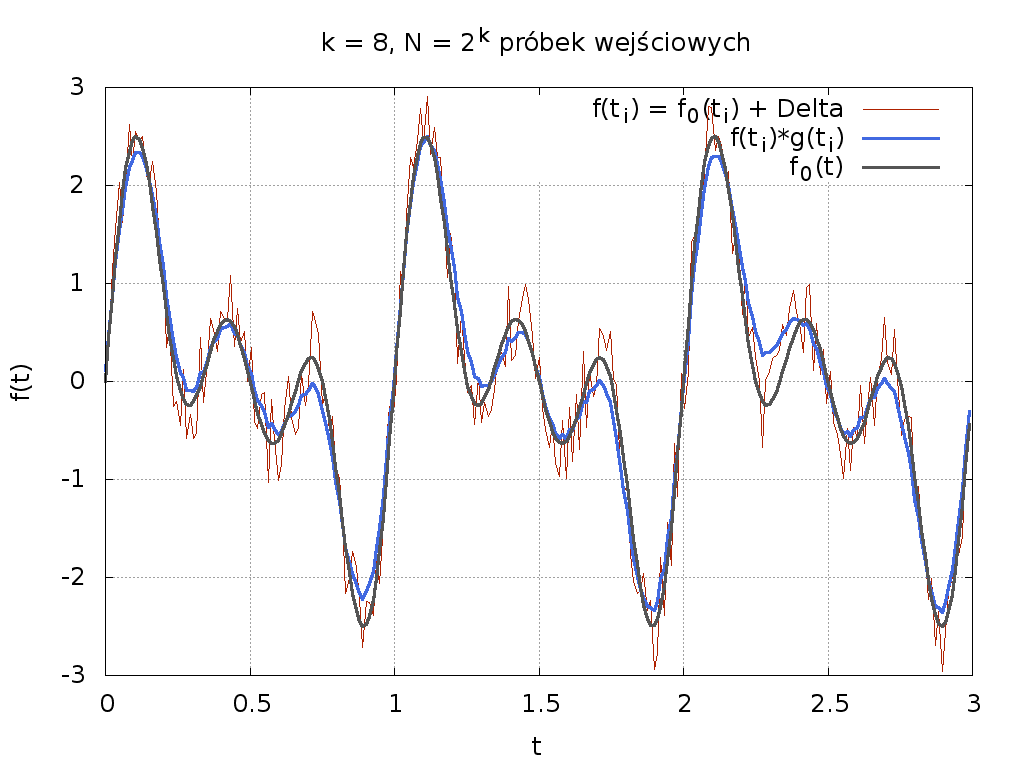
\includegraphics[height=0.41\linewidth]{k8.png}
	\caption{Wynik  odszumiania  sygnału  przy  użyciu  FFT; $  f_0(t) $ – oryginalny  sygnał  niezaburzony, $ f(t) = f0(t) + \Delta $ – sygnał zaburzony, $ f(t)\ast g(t) $ – sygnał wygładzony (odszumiony), tj. splot funkcji. Parametr $k = 8\implies N = 2^{8}$ próbek wejściowych.}
	\label{k8} 
	\end{center}
\end{figure}
\begin{figure}[h!]
	\begin{center}
	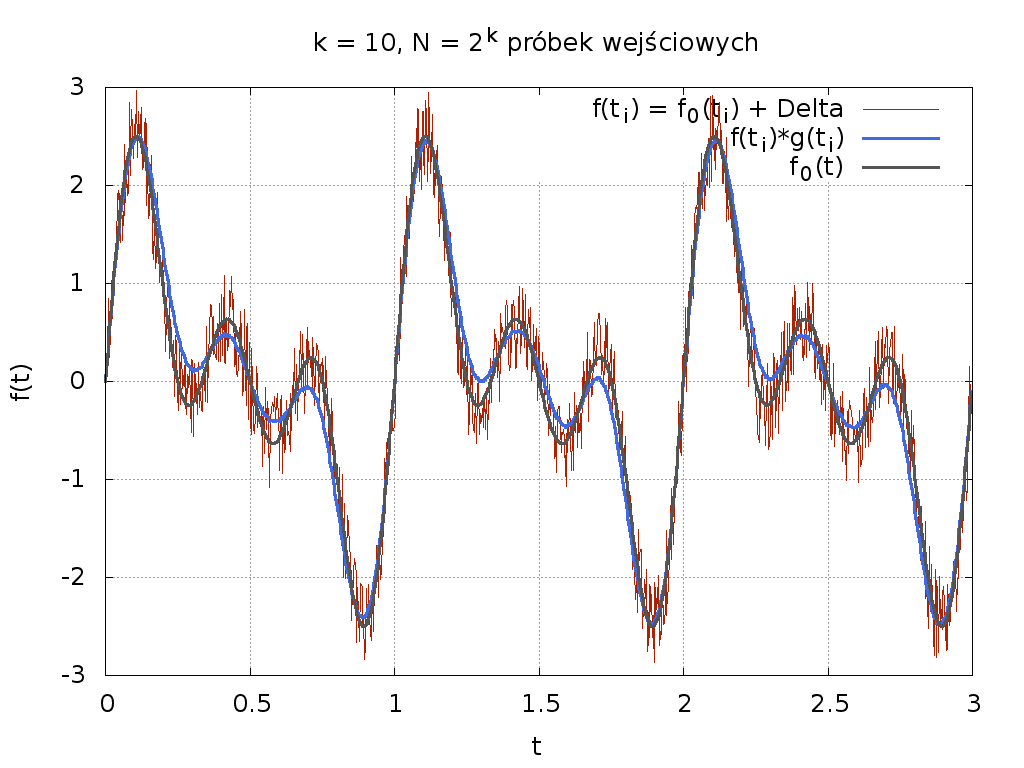
\includegraphics[height=0.41\linewidth]{k10.png}
	\caption{Wynik  odszumiania  sygnału  przy  użyciu  FFT; $  f_0(t) $ – oryginalny  sygnał  niezaburzony, $ f(t) = f0(t) + \Delta $ – sygnał zaburzony, $ f(t)\ast g(t) $ – sygnał wygładzony (odszumiony), tj. splot funkcji. Parametr $k = 10\implies N = 2^{10}$ próbek wejściowych.}
	\label{k10} 
\end{center}
\end{figure}
\begin{figure}[h!]
	\begin{center}
	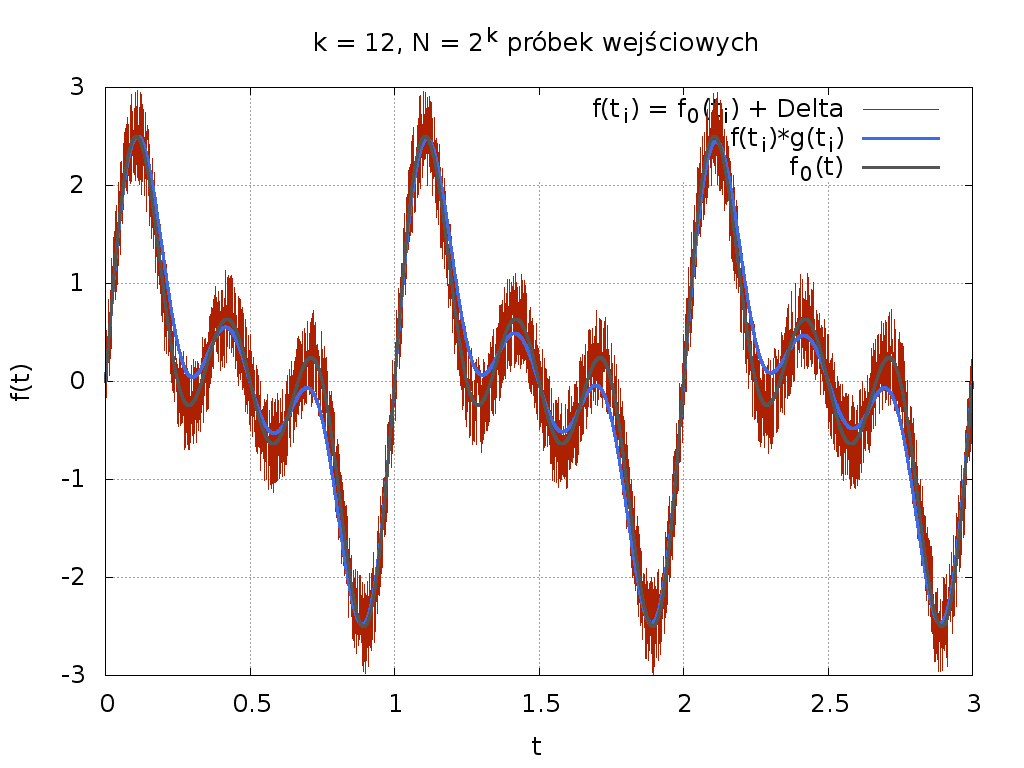
\includegraphics[height=0.41\linewidth]{k12.png}
	\caption{Wynik  odszumiania  sygnału  przy  użyciu  FFT; $  f_0(t) $ – oryginalny  sygnał  niezaburzony, $ f(t) = f0(t) + \Delta $ – sygnał zaburzony, $ f(t)\ast g(t) $ – sygnał wygładzony (odszumiony), tj. splot funkcji. Parametr $k = 12 \implies N = 2^{12}$ próbek wejściowych.}
	\label{k12} 
\end{center}
\end{figure}

\newpage
\section{Wnioski}

Analizując kolejne wykresy można dojść do wniosku, że niewystarczająca liczba próbek wejściowych nie pozwala wiernie odtworzyć pierwotnego sygnału z uwagi na brak pokrycia się ekstremów i gładkości przebiegu splotu. W przypadku (\ref{k12}) otrzymano najlepsze rezultaty, choć nieznacznie różniące się od (\ref{k10}), zatem uwypukliła się pewna granica dokładności. Zauważono ścisłą korelację między parametrem $ k $ a jakością otrzymanego wyniku, który w miarę wzrastania generował lepszy sygnał wygładzony.

Ogólnie metoda odszumiania sygnału z użyciem FFT nie pozwala uzyskać dokładnego przebiegu początkowej funkcji, a co najwyżej jego przybliżenie. Największy problem widać w okolicy wspomnianych ekstremów lokalnych. Powodów należy doszukiwać się w zadanej szerokości okna - jego poszerzenie przyczyniłoby się do lepszego pokrycia wykresów.

\end{document}